\chapter{REFERENCIAL TEÓRICO}

\section{QUALIDADE DE ENERGIA ELÉTRICA}

A definição de QEE depende muito da perspectiva. Para uma concessionária a definição se relaciona com a confiança em seu sistema elétrico, já para um fabricante é o funcionamento correto de seu equipamento com base nas características de sua fonte de alimentação \cite{ref:dugan_2004}.

Para \citeonline{ref:bollen_2003}, o termo qualidade de energia está relacionado a preocupação com desvio da tensão e corrente em relação aos valores ideais. Esses desvios são classificados em dois tipos: variações, desvios de tensões em escalas menores; e eventos, caracterizados como desvios em grande escala que acarretam interrupções.

Em consequência disso, a análise da qualidade de energia deve ser voltada para o consumidor. Portanto, um problema de qualidade de energia pode ser definido como aquele que manifesta variações de tensão, corrente ou frequência, resultando assim em uma falha ou um equipamento com mau funcionamento \cite{ref:dugan_2004}.

A QEE deve ser controlada, para que não venha a causar problemas para as cargas sensíveis dos clientes, e para que seja de fácil entendimento tanto para o fornecedor quanto para o consumidor da energia elétrica. Partindo disso, são tomados índices de qualidades de energia que estabeleçam a comparação dos níveis de tensão fornecidos pela concessionária, com os suportados pelos equipamentos do cliente \cite{ref:dugan_2004}.

\section{QUALIDADE DA ENERGIA SEGUNDO O PRODIST}

O PRODIST é a resolução normativa da ANEEL, cujo módulo 8 tem como principal objetivo estabelecer procedimentos concernentes à QEE e devem ser observados por todos que usufruem ou comercializam dessa energia \cite{ref:ANEEL2021}.

Os procedimentos que são adotados no Módulo 8, caso não possuam uma resolução específica, se aplicam ao Microssistema Isolado de Geração e Distribuição de Energia Elétrica (MIGDI) e aos Sistemas Individuais de Geração de Energia Elétrica com Fontes Intermitentes (SIGFI) \cite{ref:ANEEL2021}. Segundo o PRODIST, a QEE pode ser dividida em qualidade do produto e qualidade do serviço. A qualidade do produto, dependendo se o regime é permanente ou transitório, trata os seguintes fenômenos que afetam à qualidade da onda de tensão \cite{ref:ANEEL2021}:

\begin{itemize}
  \item Regime permanente: tensão em regime permanente; fator de potência; harmônicos; desequilíbrio de tensão; flutuação de tensão; e variação de frequência \cite{ref:ANEEL2021}.
  \item Regime transitório: variações de tensão de curta duração (VTCD) \cite{ref:ANEEL2021}.
\end{itemize}

Já a qualidade do serviço estabelece procedimentos que devem ser tomados pelas distribuidoras, com relação aos consumidores e a outras distribuidoras que venha a acessá-la \cite{ref:ANEEL2021}.

\subsection{Variações de tensão em regime permanente}

A comparação da tensão obtida por leitura com os níveis de tensão classificados como adequados, precários e críticos diz respeito a conformidade de tensão. Essa classificação deve ser obtida em torno de valores próximos a tensão de referência, conforme \autoref{fig:faixa_tensao} \cite{ref:ANEEL2021}.

\begin{figure}[H]
	\centering
	\caption{Faixas de tensão em relação à de referência}
	\label{fig:faixa_tensao}
	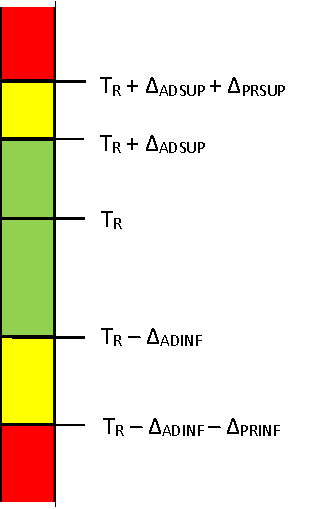
\includegraphics[width=4.4cm]{illustrations/figures/faixa_tensao.pdf}
	\fonte{\citeonline{ref:ANEEL2021}.}
\end{figure}

Em que \cite{ref:ANEEL2021}:

\begin{itemize}
  \item $T_R$ = Tensão de referência;
  \item $\Delta$ = uma variação da tensão, em que as duas primeiras letras são abreviações para a classificação de tensão e as três últimas são abreviações para inferior e superior;
  \item a cor verde corresponde a faixa adequada de tensão;
  \item em amarelo são as faixas precárias de tensão;
  \item e em vermelho são as faixas críticas de tensão.
\end{itemize}


As faixas de variação da Tensão de Leitura (TL) para pontos de conexão em tensão nominal 127V, 220V e 380V podem ser observadas na \autoref{tab:tensao_127}, \autoref{tab:tensao_220} e \autoref{tab:tensao_380} \cite{ref:ANEEL2021}.

\begin{table}[H]
  \centering
  \caption{Pontos de conexão em Tensão Nominal 127 V}
  \label{tab:tensao_127}
  \begin{tabular}{@{}cc@{}}
  \toprule
  \textbf{Tensão de Atendimento} & \textbf{Faixa de Variação da TL (Volts)} \\ \midrule
  Adequada & $117 \leq TL \leq 133$ \\
  Precária & $110 \leq TL < 117$ ou $133 < TL \leq 135$ \\
  Crítica & $TL < 110$ ou $TL > 135$ \\ \bottomrule
  \end{tabular}
  \fonte{Adaptado de \citeonline{ref:ANEEL2021}.}
\end{table}

\begin{table}[H]
  \centering
  \caption{Pontos de conexão em Tensão Nominal 220 V}
  \label{tab:tensao_220}
  \begin{tabular}{@{}cc@{}}
  \toprule
  \textbf{Tensão de Atendimento} & \textbf{Faixa de Variação da TL (Volts)} \\ \midrule
  Adequada & $202 \leq TL \leq 231$ \\
  Precária & $191 \leq TL < 202$ ou $231 < TL \leq 233$ \\
  Crítica & $TL < 191$ ou $TL > 233$ \\ \bottomrule
  \end{tabular}
  \fonte{Adaptado de \citeonline{ref:ANEEL2021}.}
\end{table}

\begin{table}[H]
  \centering
  \caption{Pontos de conexão em Tensão Nominal 380 V}
  \label{tab:tensao_380}
  \begin{tabular}{@{}cc@{}}
  \toprule
  \textbf{Tensão de Atendimento} & \textbf{Faixa de Variação da TL (Volts)} \\ \midrule
  Adequada & $350 \leq TL \leq 399$ \\
  Precária & $331 \leq TL < 350$ ou $339 < TL \leq 403$ \\
  Crítica & $TL < 331$ ou $TL > 403$ \\ \bottomrule
  \end{tabular}
  \fonte{Adaptado de \citeonline{ref:ANEEL2021}.}
\end{table}

Considerando 1008 leituras válidas com intervalos de 10 minutos, salvo as leituras expurgadas, os indicadores individuais para tensão em regime permanente são: a Duração Relativa da Transgressão de Tensão Precária (DRP) e a Duração Relativa da Transgressão de Tensão Crítica (DRC). Onde para calcular DRP e DRC segue a \autoref{eq:drp} e \autoref{eq:drc} \cite{ref:ANEEL2021},

\begin{equation}
  DRP = \frac{nlp}{1008}\cdot100,
  \label{eq:drp}
\end{equation}

\begin{equation}
  DRC = \frac{nlc}{1008}\cdot100,
  \label{eq:drc}
\end{equation}

\noindent
em que \cite{ref:ANEEL2021}:

\begin{itemize}
  \item $nlp$ = maior valor do número de leituras na faixa precária entre as fases;
  \item $nlc$ = maior valor do número de leituras na faixa crítica entre as fases.
\end{itemize}

De acordo com o módulo 8 do PRODIST, os limites para os indicadores individuais de tensão em regime permanente são \cite{ref:ANEEL2021}:

\begin{itemize}
  \item $DRP_{limite}=3\%$;
  \item $DRC_{limite}=0,5\%$.
\end{itemize}

Caso as medições obtidas estejam com DRP e DRC superiores aos delimitados pelo PRODIST, a distribuidora deve compensar o titular da unidade consumidora conforme a \autoref{eq:comp} \cite{ref:ANEEL2021},

\begin{equation}
  Comp=\left\lceil\left(\frac{DRP - DRP_{limite}}{100}\right) \cdot k_1+\left(\frac{D R C-D R C_{limite}}{100}\right) \cdot k_2\right\rceil \cdot EUSD,
  \label{eq:comp}
\end{equation}

\noindent
em que \cite{ref:ANEEL2021}:

\begin{itemize}
  \item $k_1=0$ se $DRP \leq DRP_{Limite}$ senão $k_1=3$;
  \item $k_2=0$ se $DRC \leq DRC_{Limite}$ senão: para consumidores atendidos em Baixa Tensão (BT) $k_2=7$; para consumidores atendidos em Média Tensão (MT) $k_2=5$; ou para consumidores atendidos em Alta Tensão (AT) $k_2=3$;
  \item $EUSD =$ valor do Encargo de Uso do Sistema de Distribuição, referente ao último mês colhido a medição.
\end{itemize}

\subsection{Fator de potência}

Considerando um ângulo de fase $\theta$ entre a corrente e a tensão, o cosseno desse ângulo é denominado fator de potência ($fp$). Sabe-se que, a depender do sinal de $cos\theta$, o $fp$ pode determinar se a corrente está atrasada ou adiantada em relação a tensão. Dessa forma, para um sistema no qual a corrente está atrasada em relação a tensão é dito que o fator de potência é indutivo, em contrapartida, se estiver adiantada o fator de potência é capacitivo \cite{ref:glover_2017}.

O fator de potência pode ser calculado através da \autoref{eq:fp_glover} \cite{ref:glover_2017},

\begin{equation}
  fp = \frac{P}{\sqrt{P^2 + Q^2}},
  \label{eq:fp_glover}
\end{equation}

\noindent
em que:

\begin{itemize}
  \item $P =$ potência ativa;
  \item $Q =$ potência reativa.
\end{itemize}

Uma outra forma de calcular o fator de potência é seguindo a \autoref{eq:fp_prodist}, fornecida pelo PRODIST \cite{ref:ANEEL2021},

\begin{equation}
  fp = \frac{EA}{\sqrt{EA^2 + ER^2}},
  \label{eq:fp_prodist}
\end{equation}

\noindent
em que, EA e ER são as energias ativa e reativa, respectivamente \cite{ref:ANEEL2021}.

O PRODIST determina que, para consumidores do Grupo A com tensão menor que 230 kV, o fator de potência deve estar entre 0,92 e 1,00, tanto para indutivo quanto para capacitivo \cite{ref:ANEEL2021}.

\subsection{Harmônicos}

Harmônicos são definidos como correntes ou tensões senoidais que possuem frequências com valores múltiplos da frequência fundamental de um sistema. Geralmente esses valores são múltiplos de 50 ou 60 Hz \cite{ref:fuchs_2015}. Sendo assim, para um sistema de 60 Hz que possua 5 harmônicos de ordens diferentes: 180, 300, 360, 420 e 540 Hz, respectivamente.

As principais causas de harmônicos em sistemas são \cite{ref:fuchs_2015}:

\begin{itemize}
  \item cargas não lineares, por exemplo: retificadores ou inversores;
  \item cargas residenciais, como televisores e computadores;
  \item dispositivos de controle com mau funcionamento;
  \item perdas em transformadores e capacitores;
  \item ruídos em motores.
\end{itemize}

A presença de equipamentos com características não lineares altera a forma de onda, produzindo ondas não senoidais. Essas formas de ondas podem ser expressas em séries de Fourier, em que cada termo pode representar: componentes sub-harmônicas; componente fundamental; componentes inter-harmônicas; e componentes harmônicas \cite{ref:fuchs_2015}.

Tanto para as séries de Fourier, como para os harmônicos de uma função não senoidal, existem componentes pares e ímpares que se equivalem. Quando a série de Fourier possui apenas componentes ímpares, quer dizer que o formato de onda dos semiciclos positivos e negativos são iguais. Porém quando existe a presença eventual de componentes pares, significa que pode existir algum problema no sistema \cite{ref:fuchs_2015}.

Quando há presença de harmônicos triplos, ou seja, harmônicos ímpares múltiplos de 3, significa que existe a presença de corrente na linha de neutro podendo acarretar sobrecarga do respectivo condutor \cite{ref:fuchs_2015}.

Quando há ocorrência de distorções harmônicas o formato da onda analisado possui deformações em comparação com os formatos das tensões e correntes puramente senoidais \cite{ref:ANEEL2021}.

Sendo assim, adotam-se alguns indicadores para as distorções harmônicas, nos quais, para uma ordem $h$, o indicador de distorção harmônica individual ($DIT_h\%$) pode ser calculado pela \autoref{eq:dit_h} \cite{ref:ANEEL2021},

\begin{equation}
  DIT_h\% = \frac{V_h}{V_1}\cdot 100,
  \label{eq:dit_h}
\end{equation}

\noindent
em que $V_h$ corresponde a tensão harmônica de ordem $h$ e $V_1$ é a componente fundamental da tensão \cite{ref:ANEEL2021}.

Para calcular a distorção harmônica total de tensão ($DTT\%$) usa a \autoref{eq:dtt} \cite{ref:ANEEL2021},

\begin{equation}
  DTT\% = \frac{\sqrt{\sum_{h=2}^{h_{max}}V_h^2}}{V_1}\cdot 100,
  \label{eq:dtt}
\end{equation}

\noindent
na qual $h$ corresponde as ordens harmônicas que variam de 2 até $h_{max}$ (ordem harmônica de maior valor) \cite{ref:ANEEL2021}.

Levando em consideração apenas os componentes pares não múltiplos de 3, o PRODIST determina que a distorção harmônica total de tensão ($DTT_p\%$) deve ser calculada da seguindo a \autoref{eq:dtt_p} \cite{ref:ANEEL2021},

\begin{equation}
  DTT_p\% = \frac{\sqrt{\sum_{h=2}^{h_{p}}V_h^2}}{V_1}\cdot 100,
  \label{eq:dtt_p}
\end{equation}

\noindent
sendo que, $h$ representa as ordens harmônicas pares e não múltiplas de 3, com $h_p$ sendo o maior valor da ordem harmônica \cite{ref:ANEEL2021}. Assim como para as componentes pares, as ímpares possuem um indicador de distorção harmônica total de tensão ($DTT_i\%$), determinado pela \autoref{eq:dtt_i} \cite{ref:ANEEL2021},

\begin{equation}
  DTT_i\% = \frac{\sqrt{\sum_{h=5}^{h_{i}}V_h^2}}{V_1}\cdot 100,
  \label{eq:dtt_i}
\end{equation}

\noindent
em que, $h$ simboliza as ordens harmônicas ímpares e não múltiplas de 3 partindo do 5, com $h_i$ sendo o maior valor da ordem harmônica \cite{ref:ANEEL2021}.

Por último, levando em consideração apenas as componentes múltiplas de 3, o indicador referente é determinado pela \autoref{eq:dtt_3} \cite{ref:ANEEL2021},

\begin{equation}
  DTT_3\% = \frac{\sqrt{\sum_{h=3}^{h_{3}}V_h^2}}{V_1}\cdot 100,
  \label{eq:dtt_3}
\end{equation}

\noindent
sabendo-se que, $h$ representa as ordens harmônicas múltiplas de 3, com $h_3$ como o maior valor da ordem harmônica múltipla de 3 \cite{ref:ANEEL2021}.

Levando em consideração as 1008 leituras válidas determinadas pelo PRODIST, deve ser calculado o percentil 95 para os indicadores de distorções harmônicas total de tensão. Em seguida, os valores obtidos devem ser comparados com os limites estabelecidos pelo próprio PRODIST, conforme \autoref{tab:limites_distorcoes_harmonicas}, em que $V_n$ é a tensão nominal do sistema \cite{ref:ANEEL2021}.

\begin{table}[H]
  \centering
  \caption{Limites das distorções harmônicas totais de tensão}
  \label{tab:limites_distorcoes_harmonicas}
  \begin{tabular}{@{}cccc@{}}
  \toprule
  \textbf{Indicador} & \textbf{$V_n\leq 2,3$ kV} & \textbf{$2,3$ kV $\leq V_n<69$ kV} & \textbf{$69$ kV $\leq V_n<230$ kV} \\ \midrule
  $DTT95\%$ & $10,00\%$ & 8,00\% & 5,00\% \\
  $DTT_p95\%$ & $2,50\%$ & $2,00\%$ & $1,00\%$ \\
  $DTT_i95\%$ & $7,50\%$ & $6,00\%$ & $4,00\%$ \\
  $DTT_395\%$ & $6,50\%$ & $5,00\%$ & $3,00\%$ \\ \bottomrule
  \end{tabular}
  \fonte{Adaptado de \citeonline{ref:ANEEL2021}.}
\end{table}

\subsection{Desequilíbrio de tensão}

O PRODIST define o desequilíbrio de tensão como qualquer alteração nos valores das amplitudes das tensões de fase ou na defasagem de um sistema trifásico \cite{ref:ANEEL2021}. De forma análoga, para \citeonline{ref:fuchs_2015} caso um sistema trifásico não apresente as tensões com valores iguais de amplitude e defasagem de 120 graus entre si, existe um desequilíbrio de tensão nesse sistema.

As principais consequências do desequilíbrio de tensão são mau funcionamento e danos a vida útil dos equipamentos elétricos. Já a principal fonte de desequilíbrio são as cargas elétricas, tanto as lineares (motores de indução) quanto as não lineares (conversores estáticos CA-CC) \cite{ref:paulilo_2013}.

Os dois principais tipos de origens de desequilíbrio de cargas são: estrutural e funcional. O termo estrutural diz respeito a qualquer desequilíbrio na rede, sejam transformadores ou linhas de transmissão que estejam desbalanceadas. Já funcional remete à presença de cargas desequilibradas na rede, em que as fases não estão corretamente balanceadas \cite{ref:rezende_2012}.

Para calcular o Fator de Desequilíbrio de Tensão ($FD\%$), o PRODIST segue a \autoref{eq:fd_1} \cite{ref:ANEEL2021},

\begin{equation}
  FD\% = \frac{V_-}{V_+}\cdot 100,
  \label{eq:fd_1}
\end{equation}

\noindent
em que, $V_-$ e $V_+$ são as tensões eficazes para sequência negativa e positiva, respectivamente, considerando a frequência fundamental. Alternativamente, tem-se a \autoref{eq:fd_2} \cite{ref:ANEEL2021}.

\begin{equation}
  FD\%=100 \cdot \frac{\sqrt{1-\sqrt{3-6 \beta}}}{\sqrt{1+\sqrt{3-6 \beta}}},
  \label{eq:fd_2}
\end{equation}

O valor de $\beta$ é determinado pela \autoref{eq:beta} \cite{ref:ANEEL2021},

\begin{equation}  
  \beta=\frac{V_{a b}^4+V_{b c}^4+V_{c a}^4}{\left(V_{a b}^2+V_{b c}^2+V_{c a}^2\right)^2},
  \label{eq:beta}
\end{equation}

\noindent
em que, $V_{ab}$, $V_{bc}$ e $V_{ca}$ são as tensões de linha eficazes para frequência fundamental das fases ab, bc e ca, respectivamente \cite{ref:ANEEL2021}.

Assim como os outros limites, para o PRODIST deve ser calculado o percentil 95 para os 1008 valores do $FD\%$ obtidos. Com isso, o valor limite para o $FD95\%$ pode ser observado na \autoref{tab:limites_desequilibrio_tensao}, em que $V_n$ é a tensão nominal \cite{ref:ANEEL2021}.

\begin{table}[H]
  \centering
  \caption{Limites para o indicador de desequilíbrio de tensão}
  \label{tab:limites_desequilibrio_tensao}
  \begin{tabular}{@{}ccc@{}}
  \toprule
  \textbf{Indicador} & \textbf{$V_n \leq  2,3$ kV} & \textbf{$2,3$ kV $< V_n  < 230$ kV} \\ \midrule
  $FD95\%$ & $3,00\%$ & $2,00\%$ \\ \bottomrule
  \end{tabular}
  \fonte{Adaptado de \citeonline{ref:ANEEL2021}.}
\end{table}

\subsection{Flutuação de tensão}

Quando ocorrem mudanças repentinas nos valores de pico ou eficazes da tensão, de forma sistemática ou aleatória, caracteriza-se esse fenômeno como flutuação de tensão. Para o PRODIST, os indicadores de flutuação são o $P_{st}$ e $P_{lt}$, que representam o quanto de cintilação luminosas estão relacionadas a flutuação de tensão para os períodos de 10 minutos e 2 horas, respectivamente \cite{ref:ANEEL2021}.

$P_{st}95\%$ é o indicador utilizado para verificação do desempenho do sistema, que condiz com o percentil 95 dos valores calculados para $P_{st}$ pela \autoref{eq:pst} \cite{ref:ANEEL2021},

\begin{equation}
P_{st}=\sqrt{0,0314 P_{0,1}+0,0525 P_1+0,0657 P_3+0,28 P_{10}+0,08 P_{50}},
\label{eq:pst}
\end{equation}

\noindent
em que os valores de $P$, determinam o nível de flutuação de tensão que foi ultrapassado no percentual do tempo referente ao seu indicador \cite{ref:ANEEL2021}.

O limite para o indicador de flutuação está determinado pela \autoref{tab:limites_flutuacao_tensao} \cite{ref:ANEEL2021}.

\begin{table}[H]
  \centering
  \caption{Limites para o indicador de flutuação de tensão}
  \label{tab:limites_flutuacao_tensao}
  \begin{tabular}{@{}cccc@{}}
  \toprule
  \textbf{Indicador} & \textbf{$V_n \leq  2,3$ kV} & \textbf{$2,3$ kV $< V_n  < 69 $kV} & \textbf{$69$ kV $\leq V_n  < 230$ kV} \\ \midrule
  $P_{st}95\%$ & $1,0$ pu & $1,5$ pu & $2,0$ pu \\ \bottomrule
  \end{tabular}
  \fonte{Adaptado de \citeonline{ref:ANEEL2021}.}
\end{table}

\subsection{Variação de frequência}

Para que não haja desvio da frequência do sistema em níveis fora da variação permitida, faz-se necessário que exista equilíbrio entre a geração e carga. Esse desvio pode ser proveniente de mudanças na velocidade de rotação de geradores eletromecânicos. Outros possíveis motivos de variações na frequência são falhas no sistema de transmissão de energia \cite{ref:fuchs_2015}.

Para regime permanente e condições normais, o PRODIST determina que o sistema de distribuição deve operar em níveis de frequência entre 59,9 Hz e 60,1 Hz \cite{ref:ANEEL2021}. 


\section{PYTHON}

Python é uma linguagem de programação de alto nível e interpretada, possuindo uma escrita mais simples, de fácil leitura e com uma grande variedade de módulos (bibliotecas) para execução das mais variadas tarefas. Ademais, é dotada de estruturas de dados de alto nível, como dicionários, listas e tuplas \cite{ref:borges_2014}.

Em Python, os arquivos-fonte que são importados e executados em outro arquivo Python, são denominados de módulos. A estrutura simplificada de um modulo pode ser observada na \autoref{fig:estrutura_modulo} \cite{ref:borges_2014}.

\begin{figure}[H]
	\centering
	\caption{Estrutura básica de um módulo Python}
	\label{fig:estrutura_modulo}
	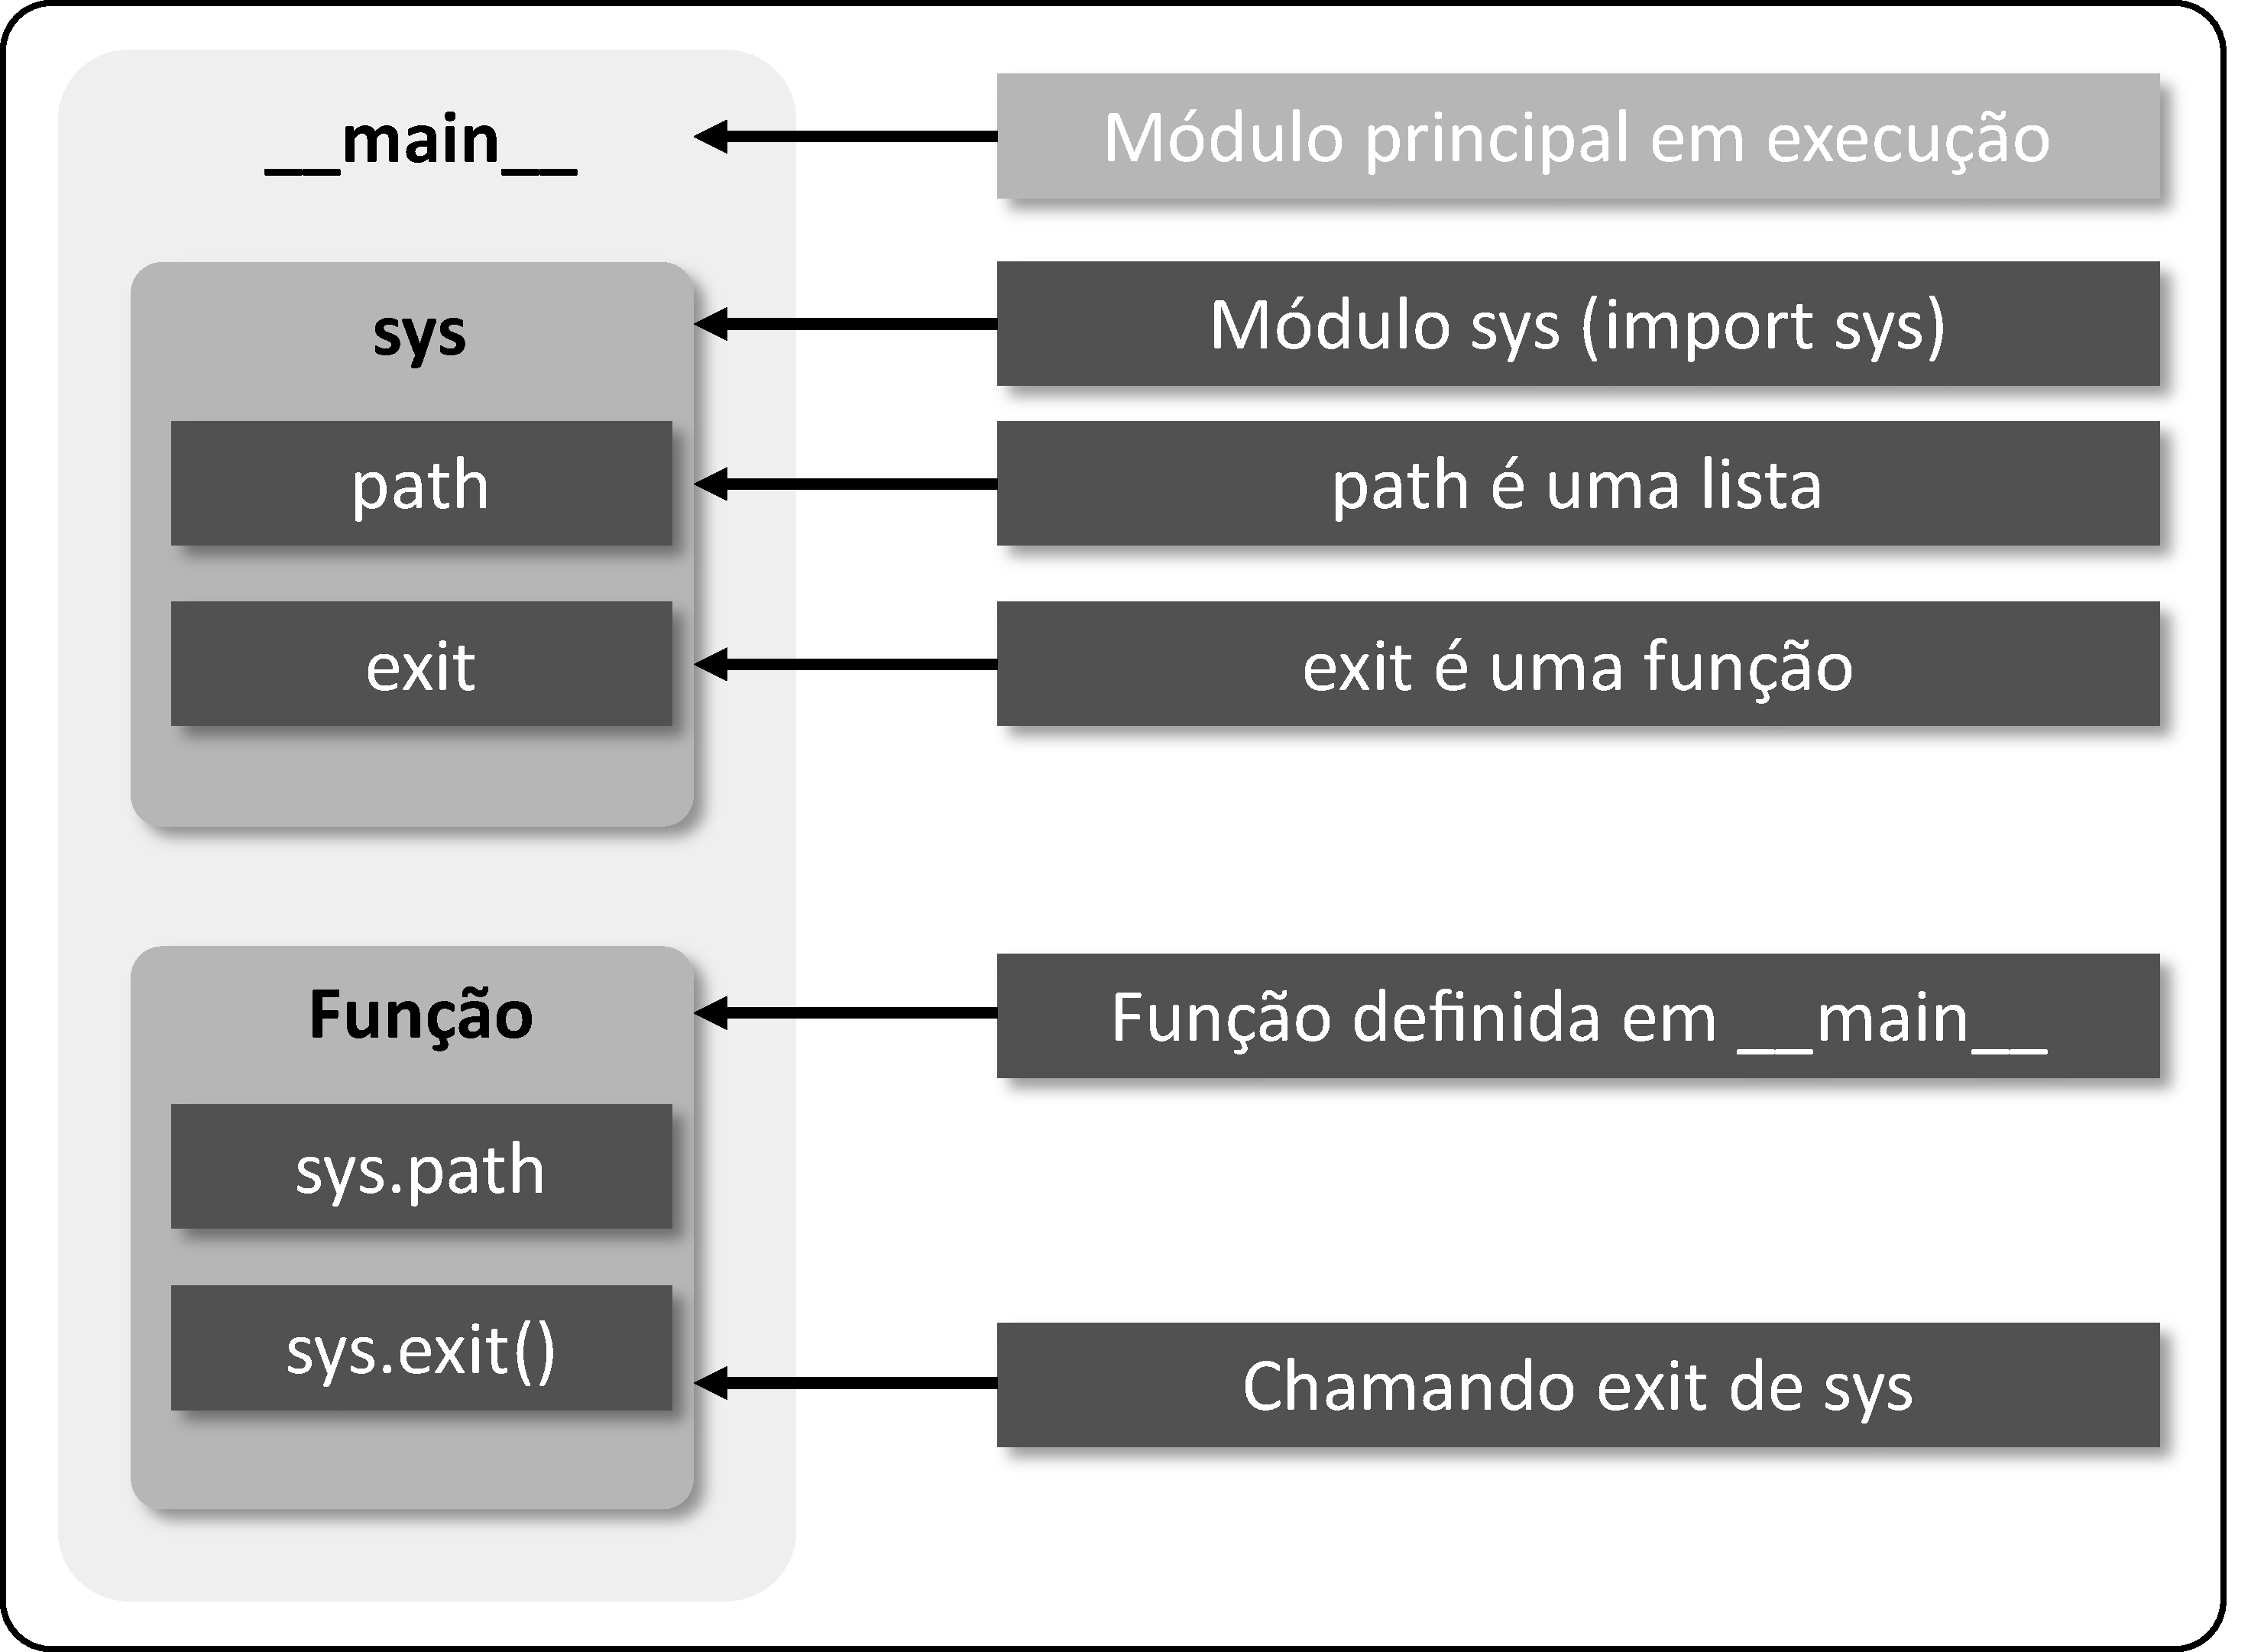
\includegraphics[width=10.8cm]{illustrations/figures/estrutura_modulo.pdf}
	\fonte{\citeonline{ref:borges_2014}.}
\end{figure}

\subsection{Análise e processamento de dados}

Quando se trata de análise e processamento de dados a linguagem Python é uma das mais utilizadas, possuindo uma grande comunidade ativa e desenvolvida na área. Um termo de grande importância é dados tabulares, também conhecido como planilhas. Por meio dos dados tabulares é possível armazenar tipos diferentes para cada coluna (string, número, data), além de salvar esses em arquivos, seja CSV ou XLS \cite{ref:mckinney_2022}.

As bibliotecas mais comuns para a análise de dados são: NumPy; Pandas; e Matplotlib \cite{ref:mckinney_2022}.

\subsection{NumPy}

A NumPy (\textit{numerc} Python) é uma biblioteca Python utilizada para cálculos numéricos, onde tem como principal objetivo trabalhar com arrays multidimensionais. A sua versão 1.0 foi lançada no final de 2006 pelo seu fundador, Travis Oliphant \cite{ref:oliphant_2006}.

Esses \textit{arrays} multidimensionais, ou \textit{ndarray} (\textit{N-dimensional array}), são objetos com um número de elementos predeterminados, no qual cada elemento possui um conjunto de vetores de mesmo tamanho e cada vetor só possui itens de mesmo tipo de dados \cite{ref:nelli_2023}.

\subsection{Pandas}

No que concerne de análise de dados, o Pandas é uma das bibliotecas mais utilizadas, principalmente por ser \textit{open source} (código aberto). Essa biblioteca foi desenvolvida por uma grande comunidade de desenvolvedores, sendo primeiramente elaborada por Wes McKinney em 2008.  Destaca-se que, em um nível mais baixo, a biblioteca utiliza-se de várias outras bibliotecas, dentre elas o NumPy \cite{ref:mckinney_2022}.

O Pandas tem como especialidade trabalhar com \textit{DataFrame} e \textit{Series}, sendo essas as duas principais estruturas de dados dessa biblioteca \cite{ref:nelli_2023}.

As \textit{Series} são objetos que representam estruturas de dados com uma dimensão, semelhante a \textit{arrays} porém com funções extras. Já os \textit{DataFrame} são objetos com estruturas de dados mais complexas, possuindo várias dimensões \cite{ref:nelli_2023}.

\subsection{Matplotlib}

A grande especialidade dessa biblioteca é desenvolver visualizações de dados em formato de gráficos em duas dimensões, podendo até desenvolver gráficos 3D. Ela consegue ter resultados similares a gráficos produzidos em \textit{softwares} como Matlab, podendo exportá-los em vários formatos como PNG, PDF, SVG e ESP \cite{ref:nelli_2023}.

Para a \textit{data science} (ciência de dados), o Matplotlib é uma das bibliotecas fundamentais em conjunto com o Pandas e NumPy, tendo ferramentas como o pyplot que tem funções com capacidade de plotar gráficos com qualidade similar ao Matlab \cite{ref:bisong_2019}.

\subsection{PySide6}

O PySide6 é a uma biblioteca feita em Python em cima da biblioteca Qt do C++, atualmente desenvolvida pela The Qt Company. Ela tem objetivo criar interfaces gráficas altamente personalizáveis e de grande versatilidade, além de ser uma biblioteca de código aberto e multiplataformas, podendo ser executada no Linux, Windows e Mac \cite{ref:fitzpatrick_2022}.
